\documentclass[xcolor=dvipsnames]{beamer}
\usepackage{subfig}
\usepackage{wrapfig}
\usetheme{Rochester}  %% Themenwahl
\usecolortheme[named=RoyalBlue]{structure}
\usebackgroundtemplate{
	\centering
	
\includegraphics[width=\paperwidth,height=\paperheight]{images/light-speed}
} 

 \addtobeamertemplate{block begin}{\pgfsetfillopacity{0.5}}{\pgfsetfillopacity{1}}
 \addtobeamertemplate{block alerted begin}{\pgfsetfillopacity{0.5}}{\pgfsetfillopacity{1}}
 \addtobeamertemplate{block example begin}{\pgfsetfillopacity{0.5}}{\pgfsetfillopacity{1}}

\setbeamertemplate{navigation symbols}{}

\title{Solve'n Slide}
\subtitle{Alpha Presentation}
\author{Hanieh Arjomand-Fard\\Kevin Sawischa\\Markus Ansorge\\Stefan Aicher}
\date{26. June 2017}

\begin{document}
	\maketitle
	
	\begin{frame}
		\frametitle{Models and Animations}
		\begin{columns}[T]
			\begin{column}{0.7\textwidth}
				\begin{itemize}
					\item Drone
					\begin{itemize}
						\item animated
					\end{itemize}
					\item Key
					\item Updated character
					\begin{itemize}
						\item now animated
					\end{itemize}
				\end{itemize}
				\begin{figure}[ht]
					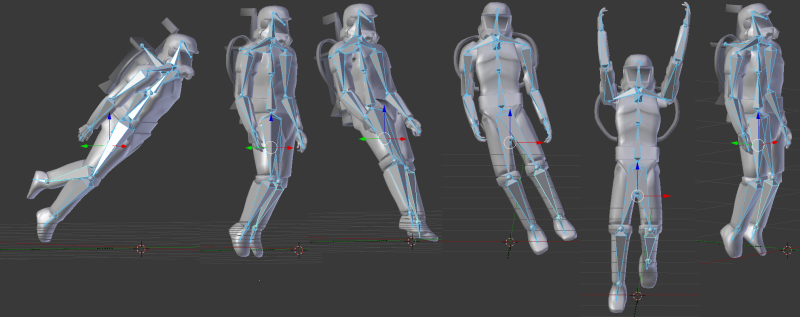
\includegraphics[scale=0.36]{images/alpha/allAnimations}
				\end{figure}
			\end{column}
			\begin{column}{0.3\textwidth}
				\begin{figure}[ht]
					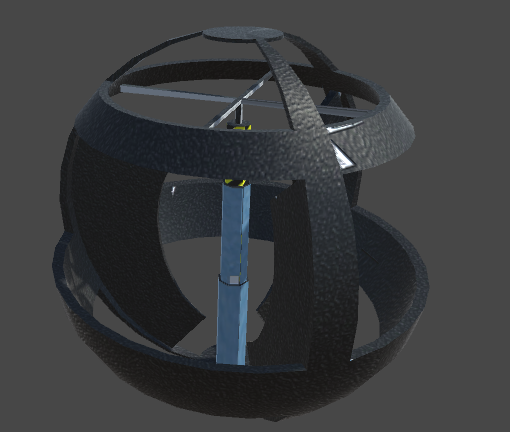
\includegraphics[scale=0.25]{images/alpha/drone}
				\end{figure}
				\begin{figure}[ht]
					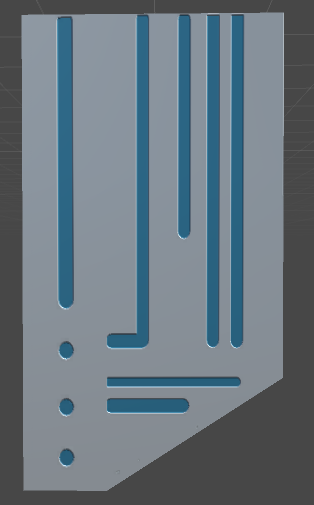
\includegraphics[scale=0.2]{images/alpha/keycardModel}
				\end{figure}
			\end{column}
		\end{columns}
	\end{frame}
	
	\begin{frame}
		\frametitle{User Interface}
		\begin{itemize}
			\item 3D main menu with freely controllable camera
			\item Icons for ingame representing charges, fueltanks and keys
			\item Bars for fuel and health
		\end{itemize}
		\begin{figure}[H]
			\centering
			\begin{tabular}{ccc}
				\subfloat{
\includegraphics[scale=.5]{images/alpha/chargeIcon}}&
				\subfloat{
\includegraphics[scale=.5]{images/alpha/fuelTankIcon}}&
				\subfloat{
\includegraphics[scale=.5]{images/alpha/keyIcon}}
			\end{tabular}
		\end{figure}
		\begin{figure}[ht]
			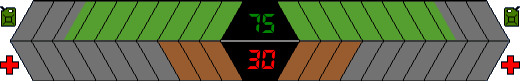
\includegraphics[scale=0.5]{images/alpha/fuelHealthBar}
		\end{figure}
	\end{frame}
	
	\begin{frame}
		\frametitle{Particle Effects}
		\begin{itemize}
			\item Using built-in particle system
			\item Finished:
			\begin{itemize}
				\item Rocket trail with fire and smoke
				\item Explosion
				\item Firework
			\end{itemize}
		\end{itemize}
		\begin{figure}[H]
			\centering
			\begin{tabular}{ccc}
				\subfloat{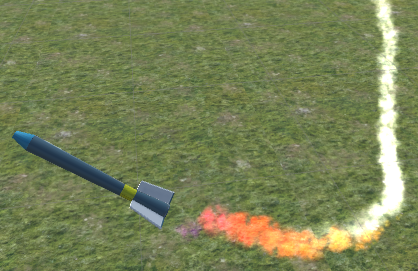
\includegraphics[scale=0.3]{images/alpha/RocketTrailFireFX}}&
				\subfloat{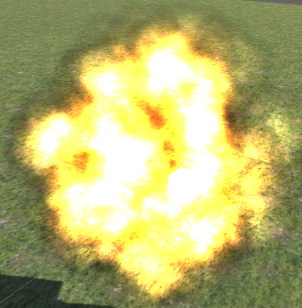
\includegraphics[scale=0.3]{images/alpha/ExplosionFX}}&
				\subfloat{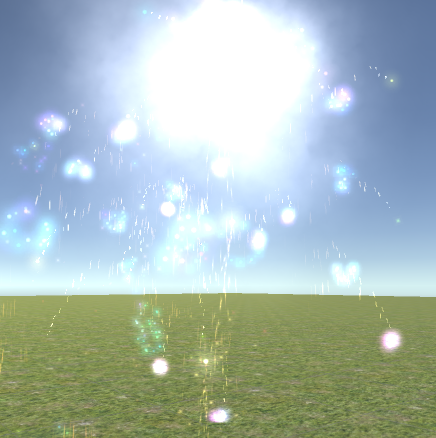
\includegraphics[scale=0.3]{images/alpha/FireworksFX}}
			\end{tabular}
		\end{figure}
	\end{frame}
	
	\begin{frame}
		\frametitle{Other Changes}
		\begin{itemize}
			\setlength\itemsep{1em}
			\item Better terrain manipulation
			\item Regain charges
			\item Fuel tanks
			\item Unmodifiable terrain
			\item Terrain characteristics
			\item Doors and keys
			\item Sound effects
		\end{itemize}
	\end{frame}
	
	\begin{frame}
		\frametitle{Demo}
		\centering
		\Huge
		Time for a live demo!
	\end{frame}
\end{document}